\mainmatter%
\setcounter{page}{1}

\lectureseries[\course]{\course}

\auth[\lecAuth]{Lecturer: \lecAuth\\ Scribe: \scribe}
\date{November 17, 2009}

\setaddress%

% the following hack starts the lecture numbering at 15
\setcounter{lecture}{14}
\setcounter{chapter}{14}

\lecture{Variance of Transfer Function Estimates}

\section{Review of Parameter Estimate Variance}
In Lecture 14 we looked at the variance of parameter estimates when $\mathcal{S}\in\mathcal{M}$ and found that $\text{cov}\{\sqrt{N}\thetan\} \sim \mathcal{N}(0,P_\theta)$ as $N\to\infty$, where $P_\theta = \lambda\bar{E}\{\psi(t,\theta_0)\psi^T(t,\theta_0)\}$ and
$$\psi(t,\theta_0) = -\left.\ptheta\epsilon(t,\theta)\right|_{\theta=\theta_0}$$
This shows how the variance changes relative to the sensitivity of the estimate with respect to the parameters and the model.
This can be estimated via
\begin{align*}
&\hat{P}_N = \hat{\lambda}\onen\sumt\psi(t,\thetan)\psi^T(t,\thetan) \\
&\hat{\lambda} = \onen\sumt\epsilon^2(t,\thetan) \\
&\thetan = \text{sol}_\theta\onen\sumt\psi(t,\theta)\epsilon(t,\theta) = 0 \\
&\ptheta\onen\sumt\epsilon^2(t,\theta) = 0
\end{align*}
Note that the last two expressions are both valid ways to solve for the estimate.
Either find the solution with respect to $\theta$ using the inner products or set the derivative to zero --- both will find a minimum.
Typically these estimates are found iteratively and can only be found directly when something like least squares or instrumental variable is able to be used.

\begin{align*}
\text{LS}: \text{sol}_\theta \onen\sumt\vp(t)\epsilon(t,\theta) = 0 \\
\text{IV}: \text{sol}_\theta \onen\sumt\xi(t)\epsilon(t,\theta) = 0
\end{align*}
Recall that for IV there is no sense of the derivative being set to zero so we do not know if we are at a minimum and there is no sense of optimality.

\begin{example}
\label{ex:15arx}
The system is given by
$$\mathcal{S}: y(t) = b_1u(t-1)-a_1y(t-1)+e(t)$$
where $u(t)\perp e(t)$, $\{e(t)\}$ is white noise with variance $\lambda$ and $\{u(t)\}$ is white noise with variance $1$.
The model is given using ARX such that
\begin{align*}
\mathcal{M}: y(t) &= bu(t-1)-ay(t-1)+\epsilon(t,\theta) \\
&= \vp^T(t)\theta+\epsilon(t,\theta) \\
&= G_\theta(q)u(t) + H_\theta(q)\epsilon(t,\theta)
\end{align*}
where
\begin{align*}
\vp = \left[\begin{array}{c} u(t-1) \\ -y(t-1) \end{array}\right], \qquad \theta= \left[\begin{array}{c} b \\ a \end{array}\right], \\ G_\theta(q) = \frac{bq^{-1}}{1+aq^{-1}}, \qquad H_\theta(q) = \frac{1}{1+aq^{-1}}
\end{align*}
We can get the solution for the parameter estimate from
\begin{align*}
\thetan &= \arg\min_\theta\onen\sumt\epsilon^2(t,\theta) \\
&= \text{sol}_\theta\onen\sumt\vp(t)\epsilon(t,\theta) = 0 \\
&= \thn = {\left[\onen\sumt\vp(t)\vp^T(t)\right]}^{-1}\left[\onen\sum\vp(t)y(t)\right]
\end{align*}
Running this experiment multiple times yields different results because $u(t)$ and $e(t)$ are white noise and will be different.
To find out how good the estimates are we can look at the covariance of the parameter estimate, $\cov\{\thn\}=$?

First, compute $\psi(t,\theta)$ as
\begin{align*}
\psi(t,\theta) &= \vp(t) = \left[\begin{array}{c} u(t-1) \\ -y(t-1) \end{array}\right]
\end{align*}
We set $\psi(t,\theta)=\vp(t)$ because the model is a linear regression.

Next, compute $P_\theta$ as
\begin{align*}
P_\theta &= \lambda\cdot \bar{E}\{\vp(t)\vp^T(t)\} \\
&= \lambda\cdot \left[\begin{array}{c c}
\bar{E}\{u(t-1)u(t-1)\} & -\bar{E}\{u(t-1)y(t-1)\} \\
-\bar{E}\{y(t-1)u(t-1)\} & \bar{E}\{y(t-1)y(t-1)\}
\end{array}\right] \\
&= \lambda\cdot \left[\begin{array}{c c}
R_u(0) & -R_{yu}(0) \\ -R_{yu}(0) & R_y(0)
\end{array}\right]
\end{align*}
This is a function of covariance functions! We know that $R_u(0)=1$ because $\{u(t)\}$ is white noise.
We also know that $R_{yu}$ contains the impulse response coefficients because $\{u(t)\}$ is white noise.
However, there is a one-step time delay so $R_{yu}(0) = 0$.
The only term left to calculate is $R_y(0)$.
\begin{align*}
&\begin{cases} R_y(0) + a_1^2R_y(0)+2a_1R_y(1) = b_1^2+\lambda \\ R_y(-1)+a_1R_y(0) = R_{yu}(0) = 0 \end{cases} \\
&\Rightarrow R_y(0) = \frac{b_1^2+\lambda}{1-a_1^2}
\end{align*}
Now we find
$$P_\theta = \lambda\cdot \left[\begin{array}{c c} 1 & 0 \\ 0 & \frac{b_1^2+\lambda}{1-a_1^2} \end{array}\right]$$
Since this is a diagonal matrix it means that the covariance of the parameters is uncorrelated, see Figure~\ref{fig:15ellipsoid}.
Notice that we will get an ellipsoid when looking at the covariance and that if there is correlation the ellipsoid will be tilted (whatever tilted means in higher dimensions).

\begin{figure}[ht!]
	\centering
	\includegraphics[width=.25\textwidth]{images/15ellipsoid}
	\caption{Ellipsoid from covariance values.}
	\label{fig:15ellipsoid}
\end{figure}

Now we can find the covariance of the parameters using $P_\theta^{-1}$ as
\begin{align*}
\cov\{\hat{b}\} &= \onen\cdot\lambda \\
\cov\{\hat{a}\} &= \onen\cdot\lambda\cdot\frac{1-a_1^2}{b_1^2+\lambda} = \frac{1-a_1^2}{N}\cdot\frac{\lambda}{b_1^2+\lambda}
\end{align*}
Remember that $\lambda = \var\{e(t)\} = $ the amount of noise on the data.
Figure~\ref{fig:15cov} shows plots of the parameter covariance as the noise increases.
Notice that $\cov\{\hat{a}\}$ settles to a limit because more noise on the data gives more information about the noise model since the $a$ term contributes to both $G_\theta$ and $H_\theta$.
For a parameter estimate to reach an asymptotic limit that parameter needs to be in both the system and the noise models.
Also notice that as $N\to\infty \Rightarrow \hat{\theta}\to\theta_0$.
$\lozenge$
\end{example}

\begin{figure}[ht!]
\centering
\subfloat[$\cov\{\hat{b}\}$.]{%
\label{fig:15covb}\includegraphics[width=0.25\textwidth]{images/15covb}
} \hfill
\subfloat[$\cov\{\hat{a}\}$.]{%
\label{fig:15cova}\includegraphics[width=0.25\textwidth]{images/15cova}
}
\caption{Covariance of the parameter estimates.}
\label{fig:15cov}
\end{figure}

\section{Variance of Transfer Function Estimates}
We have seen so far that
$$\cov\{\thetan\}\sim\mathcal{N}(0,P_\theta), \qquad P_\theta = \lambda{\left[\bar{E}\{\psi(t,\theta)\psi^T(t,\theta)\}\right]}^{-1}$$
We are also interested in what happens to $\cov\{G_{\thetan}(e^{i\w})\}$ and $\cov\{H_{\thetan}(e^{i\w})\}$.
Using the system identification toolbox in \textsc{Matlab} we can plot the Bode response and get error bars such as those shown in Figure~\ref{fig:15bode1}.

\begin{figure}[ht!]
\centering
\includegraphics[width=.25\textwidth]{images/15bode1}
\caption{Sample Bode plot with error bars.}
\label{fig:15bode1}
\end{figure}

The main idea here is that we want to set up the transfer functions as
$$T(q,\theta) = \left[\begin{array}{c c} G(q,\theta) & H(q,\theta) \end{array}\right]$$
and look at $\cov\{T (e^{i\w})\}$.
We already know $\cov\{\thetan\}$, so what is the variance of the entire model? We will estimate the model with a Taylor series expansion such that
$$\hat{T} (e^{i\w},\theta) \approx~T^\ast(e^{i\w}) + \left.\ptheta~T (e^{i\w},\theta)\right|_{\theta=\theta^\ast} (\hat{\theta}-\theta^\ast)$$
The Ljung textbook has some worked examples using different models to highlight this idea.

\section{Transfer Function Variance}
We now have
\begin{align*}
&\sqrt{N}\left[\hat{T}(e^{i\w},\theta) - T(e^{i\w},\theta^\ast)\right] \sim \mathcal{N}(0,P(\w)) \\
&P(\w) = \left.\ptheta T(e^{i\w},\theta)\right|_{\theta=\theta^\ast} P_\theta {\left[\left.\ptheta T(e^{i\w},\theta)\right|_{\theta=\theta^\ast}\right]}^T
\end{align*}
Another interesting result from Ljung is that for the system
$$\mathcal{S}: y(t) = G_0(q)u(t)+v(t), \qquad v(t) = H_0(q)e(t)$$
we look at what happens as both $N\to\infty$ and $n\to\infty$ but $n<N$ (where $n$ is the model order).
Then we see that
\begin{align*}
\cov\{\hat{G}(e^{i\w})\} &\approx \frac{n}{N}\frac{\Phi_v(\w)}{\Phi_u(\w)} = \frac{n}{N}\frac{\lambda|H_0(e^{i\w})|^2}{\Phi_u(\w)} \\
\cov\{\hat{H}(e^{i\w})\} &\approx \frac{n}{N}\frac{\Phi_v(\w)}{\lambda} = \frac{n}{N}|H_0(e^{i\w})|^2
\end{align*}
The idea that $n\to\infty$ will not happen in practice because we can't find a minimum with non-linear optimization with that many parameters.
However, it is still nice to understand what happens as the model order increases.
This can be interpreted as
\begin{itemize}
\item $\cov\{\hat{G}\}$ is determined by the signal-to-noise ratio for each frequency.
\item $\cov\{\hat{H}\}$ is determined by $H_0$ itself.
\end{itemize}

\begin{example}
We can draw the transfer function estimates and their variances as $N\to\infty$ and $n\to\infty$, see Figures~\ref{fig:15tf} and~\ref{fig:15phi}.
The variance is still there at higher frequencies because we are looking at a log scale.
$\lozenge$
\end{example}

\begin{figure}[ht!]
\centering
\subfloat[Bode plot of transfer functions.]{%
\label{fig:15tfs}\includegraphics[width=0.25\textwidth]{images/15tfs}
} \hfill
\subfloat[Bode plot with variances.]{%
\label{fig:15tfvar}\includegraphics[width=0.25\textwidth]{images/15tfvar}
}
\caption{Bode plots.}
\label{fig:15tf}
\end{figure}

\begin{figure}[ht!]
\centering
\includegraphics[width=.15\textwidth]{images/15phi}
\caption{Spectrum of white-noise input.}
\label{fig:15phi}
\end{figure}

\subsection{Designing Input Signals}
Knowing this, what would a good input signal look like? Or, what would be a good $\Phi_u(\w)$ so that the variance on $\hat{G}$ is equal over all frequencies.

We could try white noise plus the noise spectrum where $\Phi_u(\w)=\lambda+\Phi_v(\w)$.
Mostly, we want to generate more data where more noise occurs in order to get a better noise model.

We could also try
$$\Phi_u(\w) = \frac{\lambda+\Phi_v(\w)}{|G_0(e^{i\w})|^2}$$
Why would we want to divide by the size of the transfer function here? We would lose any smaller resonant modes or oscillations at frequencies away from the dominant mode.
Typically, we do not want to excite the resonant modes much at all.

Note that this is normally an iterative process where we guess a model, run an experiment to identify a better estimate of the model, design the new experiment input from the better model, get a better model from the new experiment, etc.

\section{Another Use of Model Variance}
We can use
$$\hat{G}(e^{i\w}) + \var\{\hat{G}(e^{i\w})\}$$
Instead of only a nominal model, we can estimate a set (or family) of models.
This is called the uncertainty model.
$$\mathcal{G} = \left\lbrace G~|~\hat{G}+\Delta,~\Delta=3\cdot\sqrt{\var\{\hat{G}\}}\right\rbrace$$

\begin{figure}[ht!]
\centering
\includegraphics[width=.3\textwidth]{images/15bd}
\caption{Block diagram of feedback system with reference point.}
\label{fig:15bd}
\end{figure}

\subsection{Small Gain Theorem}
\label{sec:15sgt}
Using Figure~\ref{fig:15bd} how do we check the stability of the model? We can use the small gain theorem.
From Figures~\ref{fig:15sgtbd} and~\ref{fig:15sgt} we see that
\begin{align*}
||\Delta M||_\infty &< 1 \\
||\Delta M||_\infty &< ||\Delta||_\infty||M||_\infty < 1 \\
\Rightarrow ||M||_\infty &< \frac{1}{||\Delta||_\infty}
\end{align*}
In Figure~\ref{fig:15bd} we can check
$$\left|\left|\frac{C}{1+GC}\Delta\right|\right|_\infty < 1$$
for stability.

\begin{figure}[ht!]
\centering
\includegraphics[width=.1\textwidth]{images/15sgtbd}
\caption{Block diagram for small gain theorem.}
\label{fig:15sgtbd}
\end{figure}

We want to make the uncertainty, $\Delta$, small around the bandwidth of the control poiont. We can handle more uncertainty away from the control point.

\begin{figure}[ht!]
\centering
\subfloat[Separate transfer function responses.]{%
\label{fig:15sgt1}\includegraphics[width=0.25\textwidth]{images/15sgt1}
} \hfill
\subfloat[Combined transfer function response.]{%
\label{fig:15sgt2}\includegraphics[width=0.25\textwidth]{images/15sgt2}
}
\caption{Transfer functions for small gain theorem.}
\label{fig:15sgt}
\end{figure}
